\chapter{总结}

\section{项目中遇到的问题及解决方法}

\section{项目开发过程}
\subsection{项目共享仓库}
我们对于本实践项目使用 GITHUB 进行仓库共享,让每一名组员可以在该仓库上进行代码的修改以及同步,大幅度增加实践效率。通过以下网址,可以游览到本项目的共享仓库页面:https://github.com/stainsatin/elm
\begin{figure}[htbp]
    \centering
    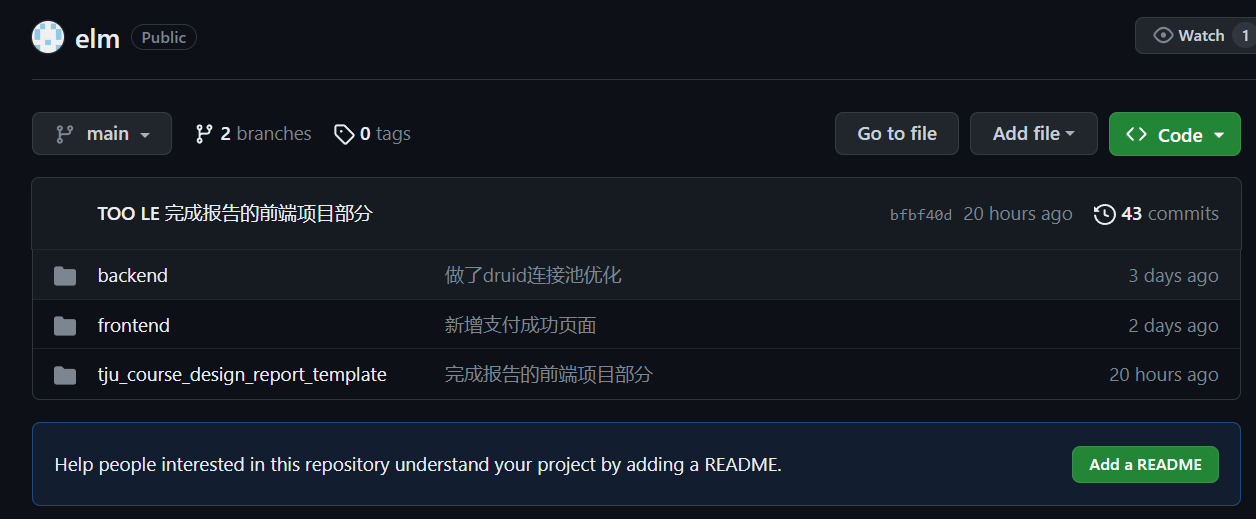
\includegraphics[width=0.8\textwidth]{githubmain}
    \caption{GITHUB 共享仓库页面}\label{fig:githubmain}
    \vspace{\baselineskip}
\end{figure}

本次实践项目的共享仓库于 8 月 23 日创建,仓库里的成员包括我们每一名组员。如上图~\ref{fig:githubmain}~所示,仓库里的内容包括本次实践项目的前端、后端与实践报告的目录,且我们每一名组员都在此共享仓库上进行了多次代码的复制和提交。经过三个星期的项目开发,以下是我们的共享仓库数据视图,如图~\ref{fig:commit}~至图所示:

\begin{figure}[htbp]
    \centering
    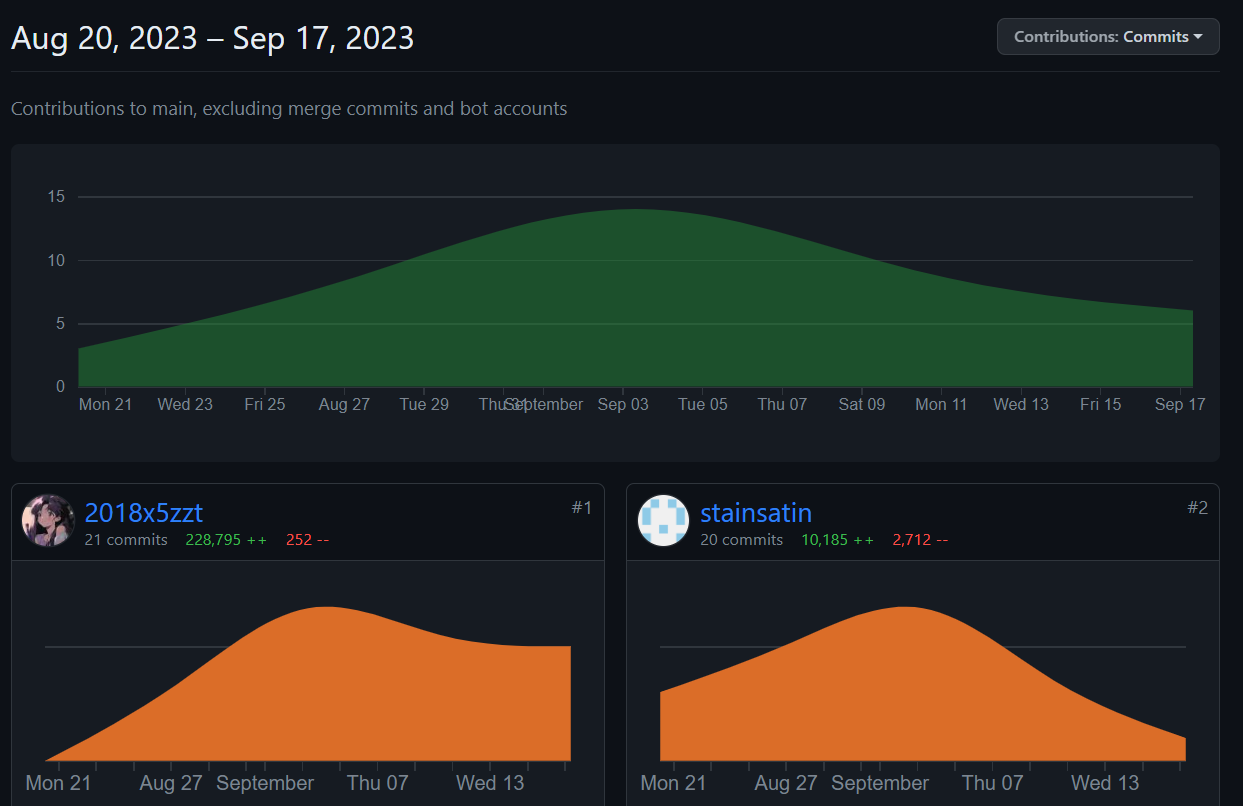
\includegraphics[width=0.7\textwidth]{commit}
    \caption{GITHUB 共享仓库提交视图}\label{fig:commit}
    \vspace{\baselineskip}
\end{figure}
\begin{figure}[htbp]
    \centering
    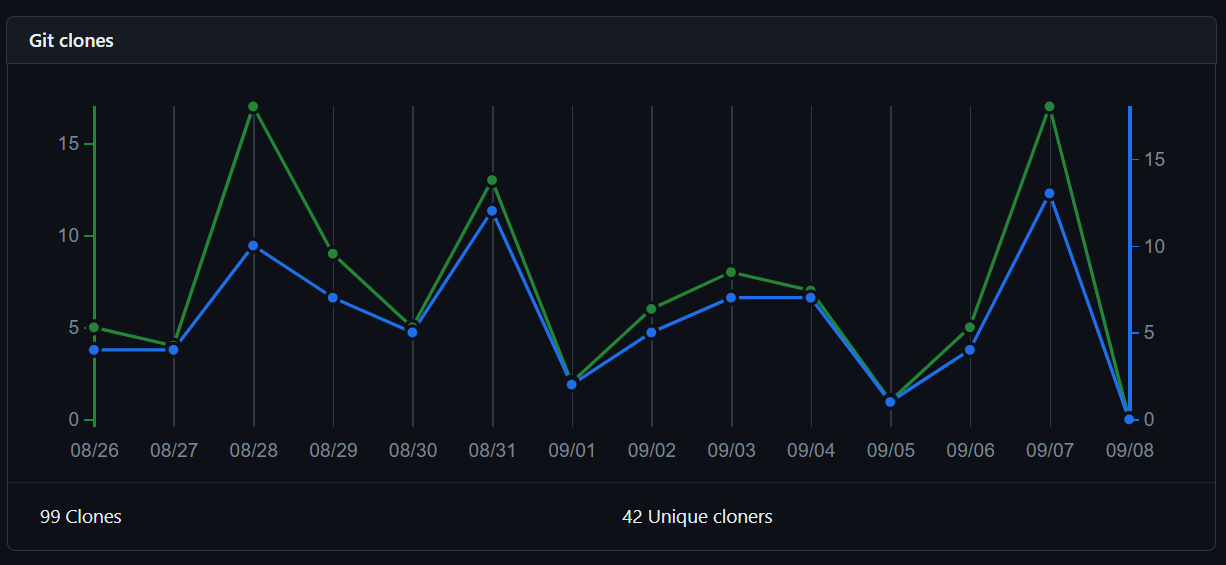
\includegraphics[width=0.8\textwidth]{clone}
    \caption{GITHUB 共享仓库复制视图}\label{fig:clone}
    \vspace{\baselineskip}
\end{figure}
\begin{figure}[htbp]
    \centering
    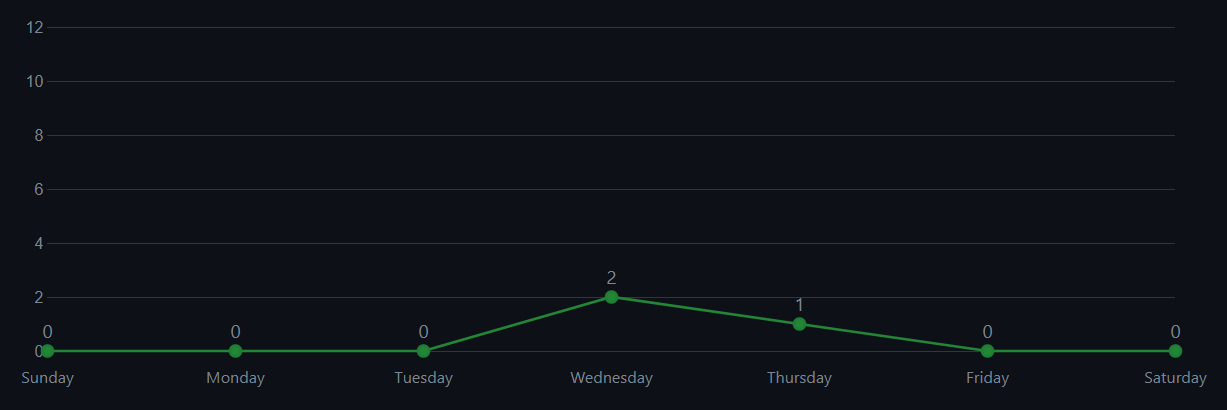
\includegraphics[width=0.8\textwidth]{week1commit}
    \caption{GITHUB 共享仓库第一周提交次数视图}\label{fig:week1commit}
    \vspace{\baselineskip}
\end{figure}
\begin{figure}[htbp]
    \centering
    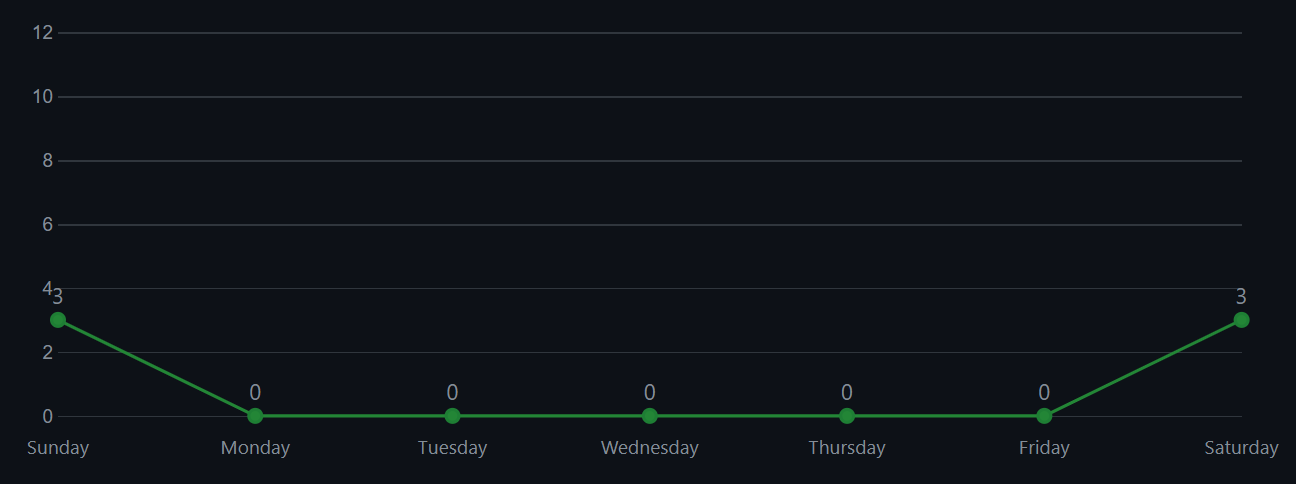
\includegraphics[width=0.8\textwidth]{week2commit}
    \caption{GITHUB 共享仓库第二周提交次数视图}\label{fig:week2commit}
    \vspace{\baselineskip}
\end{figure}
\begin{figure}[htbp]
    \centering
    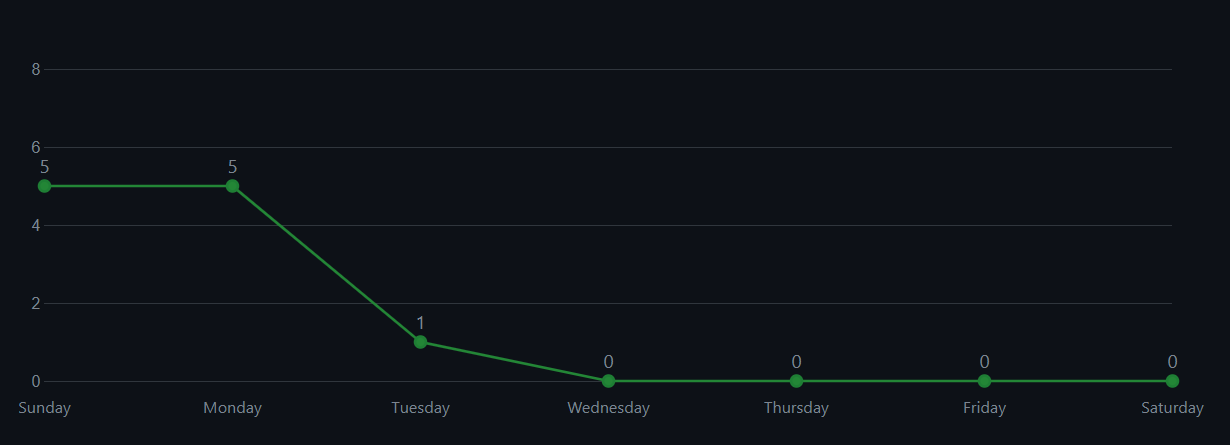
\includegraphics[width=0.8\textwidth]{week3commit}
    \caption{GITHUB 共享仓库第三周提交次数视图}\label{fig:week3commit}
    \vspace{\baselineskip}
\end{figure}
\begin{figure}[htbp]
    \centering
    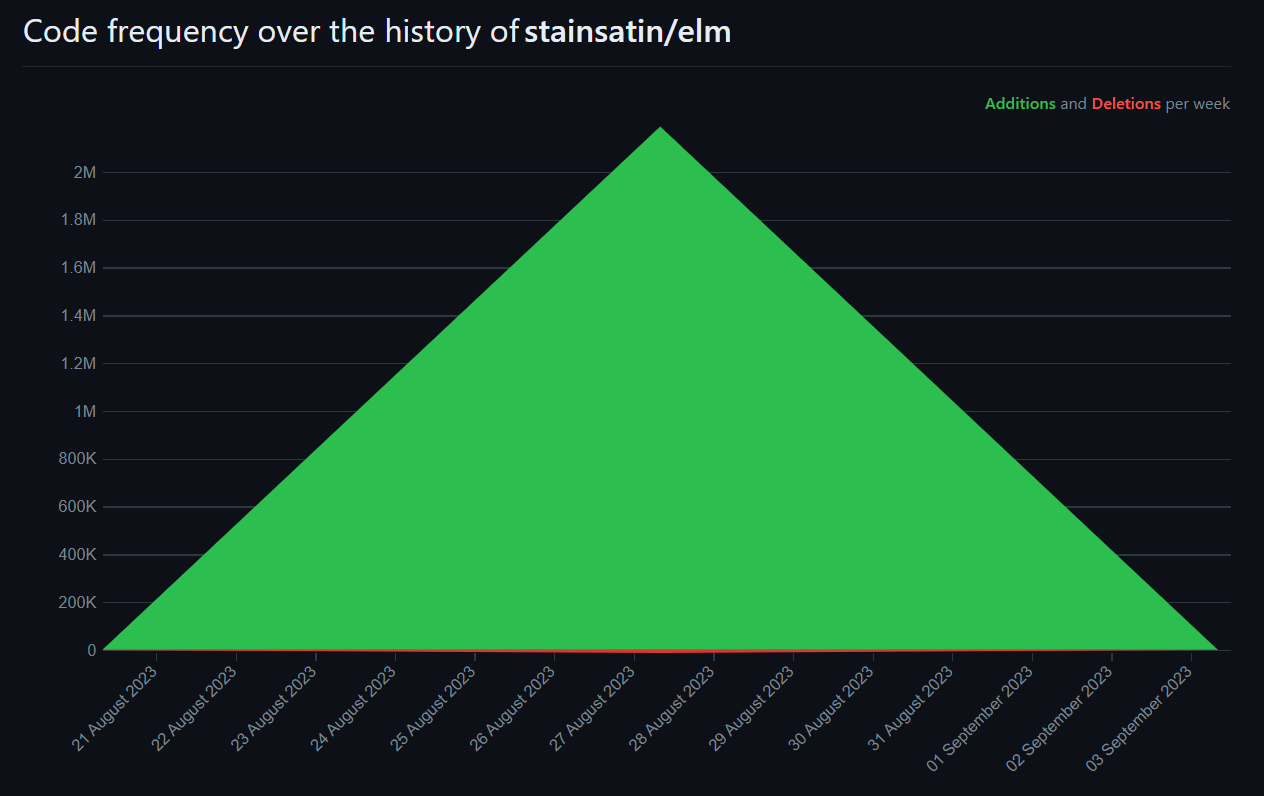
\includegraphics[width=0.7\textwidth]{codefrequency}
    \caption{GITHUB 共享仓库代码频率视图}\label{fig:codefrequency}
    \vspace{\baselineskip}
\end{figure}